
% ----------------------------------------------------------------------
\section{Climate forcing}
\label{sec:climate}
% ----------------------------------------------------------------------

We force PISM with temperature and precipitation data from one observational dataset, three global and one regional reanalyses. Here we present this climate data and describe how we use it as a forcing.

\subsection{Observation data}

WorldClim is a high-resolution climate dataset built from observation data \citep{data:worldclim}. These climate surfaces were generated by spatial interpolation between a large set of weather stations over global land areas, using 30\,arc\,s-aggregated hole-filled SRTM elevation data. This provides a resolution much higher than attained by general circulation models.

\begin{figure*}[t]
	\vspace*{2mm}
	\begin{center}
		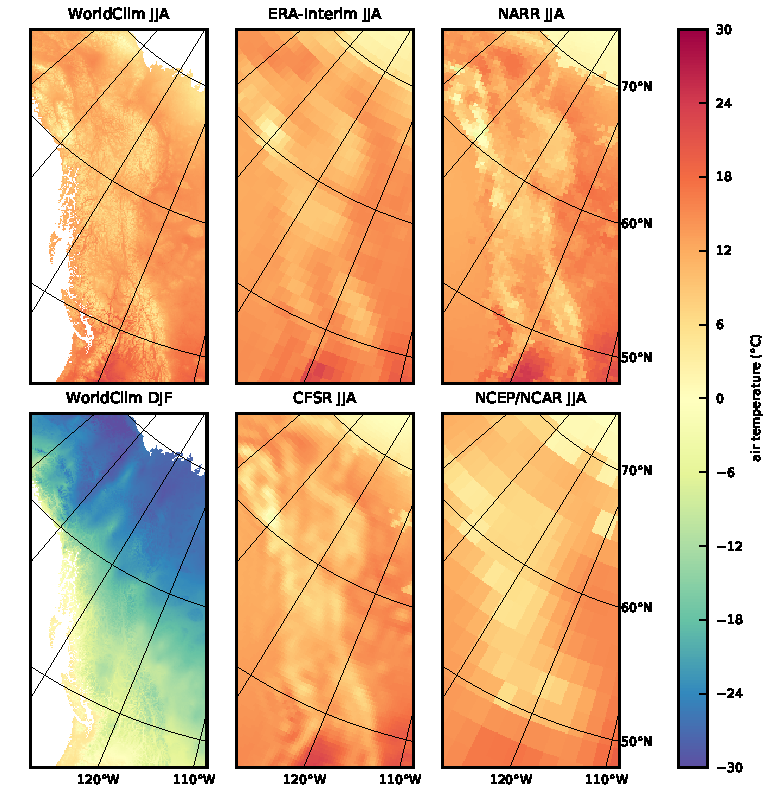
\includegraphics[width=13cm]{cordillera-climate-temp}
	\end{center}
	\caption{Summer temperature maps from the five datasets used in this study and winter temperature map from the WorldClim dataset.}
	\label{fig:temp}
\end{figure*}

Figure~\ref{fig:temp} shows the spatial distribution of summer (JJA) and winter (DJF) air surface temperatures in WorldClim. Temperatures generally decrease from south to north and regions further inland experience colder winters. It should be noted that the temperature gradient is much stronger in the winter than it is in the summer. Temperature reach well above zero during the summer months over the entire modelling domain, except of the highest peaks. In other words, there is a strong contrast in seasonality between coastal and inland regions, even and regions where mean annual temperatures are well below freezing do experience warm summers.

\begin{figure*}[t]
	\vspace*{2mm}
	\begin{center}
		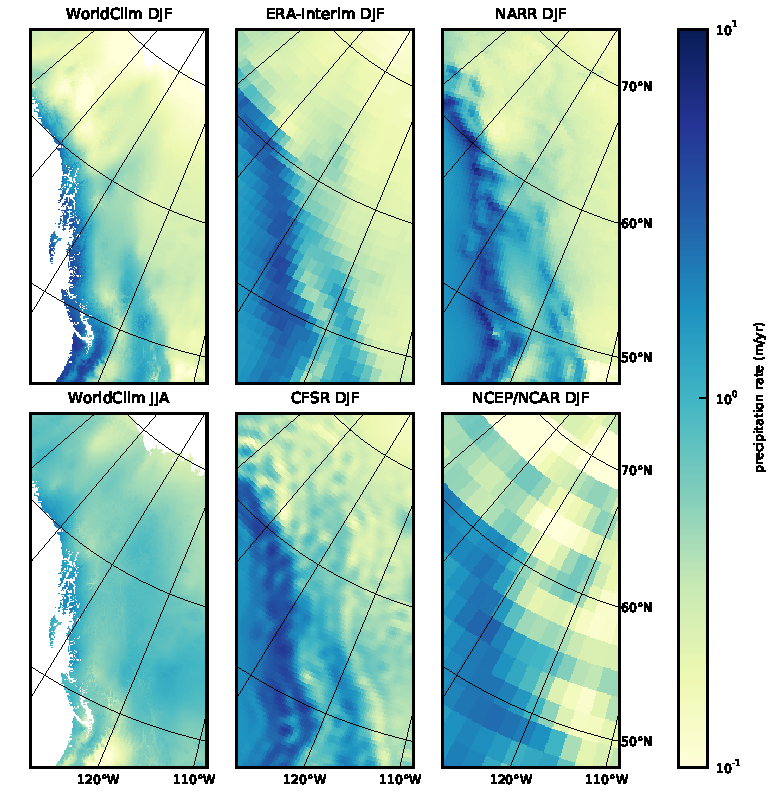
\includegraphics[width=13cm]{cordillera-climate-prec}
	\end{center}
	\caption{Winter precipitation rate maps from the five datasets used in this study and summer precipitation map from the WorldClim dataset.}
	\label{fig:prec}
\end{figure*}

Figure~\ref{fig:prec} shows the spatial distribution of DJF and JJA precipitation rates in WorldClim. Coastal regions generally receive much more precipitation than inland ones as a result of the continuous orographic barrier formed by the Boundary Ranges, the Coast Mountains and the Cascades. From a glacier mass-balance point of view, this contrast is made even stronger by the difference in timing of the precipitation peak through the year. Although coastal regions experience most precipitation as snow during the accumulation season, inland regions experience dry winters and most of the precipitation falls as rain during the summer months.

In regions like Northern Yukon and Alaska, dry winters and warm summers are unfavourable conditions to ice accumulation and glacial inception despite of the strongly negative present mean annual temperatures. In order to account for these strong gradients in seasonality, we use monthly averages of temperature and precipitation to drive the ice sheet model.

The density of weather stations used by WorldClim in the Northern American Cordillera is highly inhomogeneous. If good coverage exists in the southern parts of our modelling domain, several hundred kilometres can separate neighbouring stations in the north \citep{data:worldclim}. A second drawback of the dataset in the scope of this study is the lack of data across oceans, particularly on the Pacific continental shelf where glaciers have advanced during the last glacial cycle \citep{jackson-clague-1991}.

% ----------------------------------------------------------------------

\subsection{Reanalysis data}

\begin{table*}[t]
	\caption{Characteristic of reanalysis climatologies used to force the ice sheet model.}
	\label{tab:reanalyses}
	\vskip4mm
	\centering
	\begin{tabular}{lllll}
		\tophline
		Reanalysis& Spatial coverage& Averaging period& Resolution& Description\\
		\middlehline
		NCEP/NCAR&  global&     1981 -- 2010& 1.875\degree& \citet{data:ncar}\\
		ERA-Interim&global&     1979 -- 2011& 1.000\degree& \citet{data:erai}\\
		CFSR&       global&     1979 -- 2010& 0.325\degree& \citet{data:cfsr}\\
		NARR&       North America& 1979 -- 2000& 32\,km& \citet{data:narr}\\
		\bottomhline
	\end{tabular}
\end{table*}

Apart from the WorldClim data, we use surface air temperatures and precipitation rates from three global and one regional climate reanalyses to force the ice sheet model: the NCEP/NCAR reanalysis, the ERA-Interim reanalysis, the Climate System Forecast Reanalysis (CFSR) and the North American Regional Reanalysis (NARR). Monthly climatologies from NCEP/NCAR and NARR reanalysis were provided by the NOAA/OAR/ESRL Physical Sciences Division, Boulder, Colorado, USA, from their website at \url{http://www.esrl.noaa.gov/psd/} whereas monthly climatologies from the ERA-Interim and CFSR reanalyses were computed from their monthly mean time series. Further information on the data used is gathered in Table \ref{tab:reanalyses}.

The spatial distribution of JJA air surface temperatures and DJF precipitation rates from the four reanalyses datasets are shown in Figures~\ref{fig:temp} and~\ref{fig:prec}. Summer temperature and winter precipitation are most relevant to the glacier model as they respectively drive summer melt and winter accumulation.

As a mixed product from observations and circulation modelling, we believe that reanalysis may perform best in sparsely monitored regions such as the northernmost American Cordillera.

% ----------------------------------------------------------------------

\subsection{Preprocessing and lapse-rate corrections}

Air surface temperature and precipitation from the WorldClim data, the NCEP/NCAR, ERA-Interim, CFSR and NARR reanalyses were re-projected to Canadian Atlas Lambert conformal conic projection (EPSG code~3978) and bilinearly interpolated to the model resolution of 10\,km. In addition, WorldClim data was extrapolated to oceans using a nearest-neighbour approach. These last two steps are not presented on figures~\ref{fig:temp} and~\ref{fig:prec}.

For the CFSR, an alternative forcing was prepared by smoothing the precipitation field in order to correct for artefacts seen in figure~\ref{fig:prec}. This was done by averaging data locally in a circular neighbourhood of 7\,pixels in diameter prior to re-projection. Yet we will show that this smoothing has very limited effect on the ice sheet model outcome. These preprocessing steps were made in GRASS~GIS.

\begin{figure*}[t]
	\vspace*{2mm}
	\begin{center}
		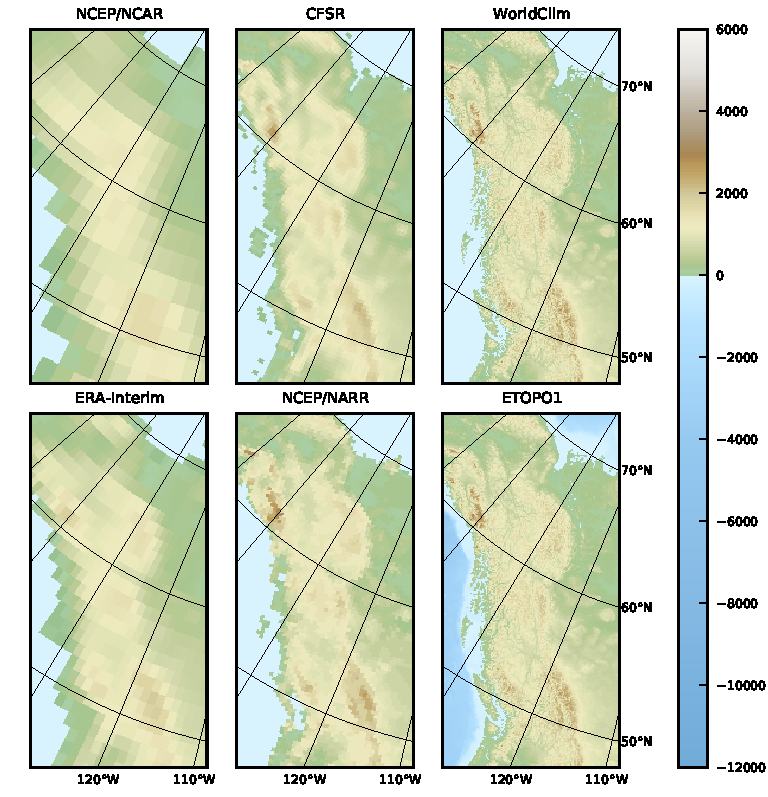
\includegraphics[width=13cm]{cordillera-climate-topo}
	\end{center}
	\caption{Reference topography used for temperature lapse-rate corrections from the five climate datasets used in the study and ETOPO1 topography used as basal condition for the ice flow model.}
	\label{fig:topo}
\end{figure*}

Throughout the simulation, the numerical model dynamically applies temperature lapse-rate corrections that account for differences between the climate forcing reference topography and the ice flow model topography on the one hand, and the evolution of ice thickness on the over hand. For reanalysis data, the circulation model surface topography (or surface geopotential height) was used as reference topography. For the WorldClim data, the aggregated hole-filled SRTM altitude field is used as reference topography. As a basal condition for the ice flow model, we use the ETOPO1\citep{data:etopo1} combined topography and bathymetry dataset. The reference topographies from the five forcing datasets, alongside the ETOPO1 data are shown in figure~\ref{fig:topo}. A lapse-rate of 6\unit{\degree C\,km^{-1}} is used in all simulations. No lapse-rate corrections apply to precipitation rates.

